%---------------------------------------------------------------------------------
%                西南交通大学研究生学位论文:第三章内容
%---------------------------------------------------------------------------------
\chapter{模板答疑}

\section{问题反馈}
\label{sec:contact}
本章节罗列了一些常见问题,供使用者参考(欢迎更多的问题反馈,一同完善本模板,受益更多的SWJTUer)。

\section{问题回答}
本部分是一个将会持续更新的版块,主要在此罗列一些在使用本模板过程中遇到的问题反馈,同时给出作者的更新或者回答,以完善swjtuThisis模板,并供后续使用的同学进行参考。

\subsection{模板问题}
\begin{enumerate}
	\item[Q1:]为什么论文编译出来的.pdf文件中所有超链接都带有颜色?
	\item[A1:]方便调试的时候区分超链接和普通文本,在main.tex文件中可以修改,详情见代码注释。
	\item[Q2:]Windows端采用CTex发行版进行论文撰写,使用内置的WinEdt编辑器打开main.tex文件时出现如图\ref{Q151208_1_Yang}所示的报错问题。
	\begin{figure}[htbp]
		\centering
		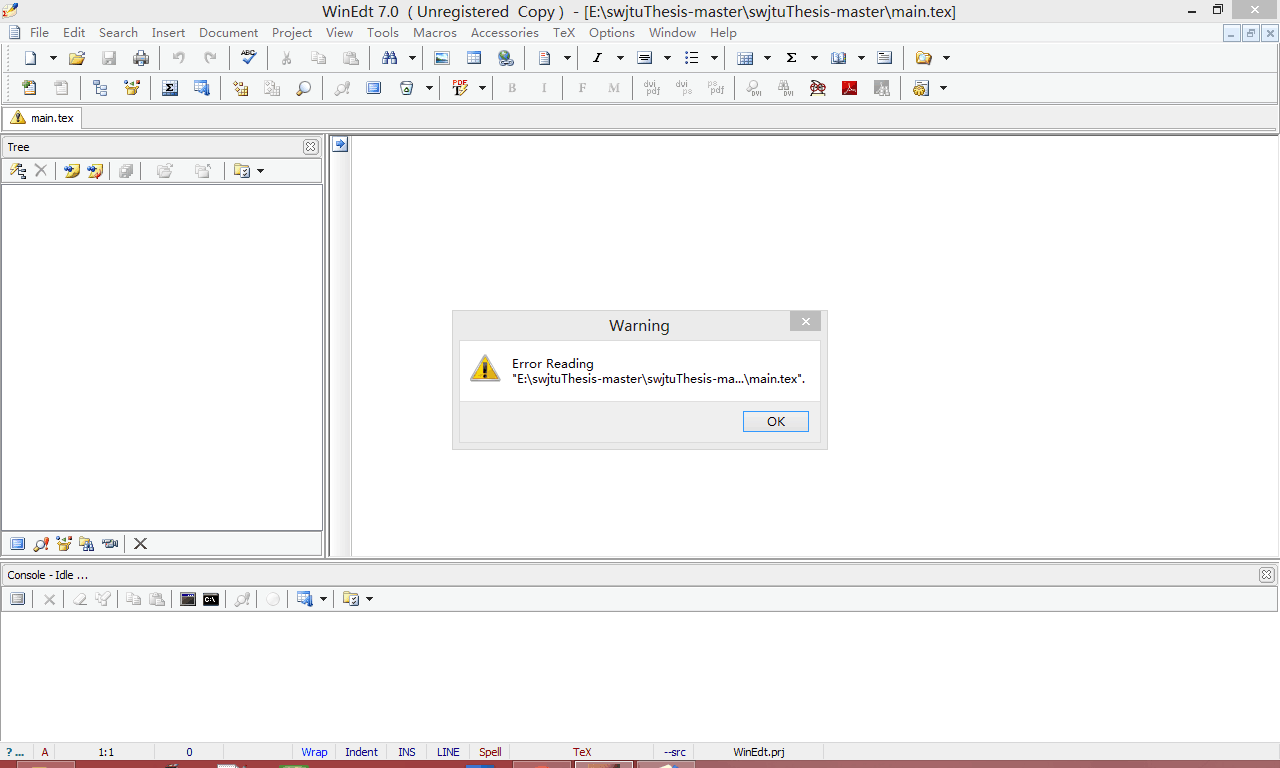
\includegraphics[width=4in]{figures/QA/Q151208_1_Yang.png}
		\caption{WinEdt打开main.tex报错}
		\label{Q151208_1_Yang}
	\end{figure}
	\item[A2:]本问题是由WinEdt编辑器内部的打开编码与模板编码不统一导致。由于swjtuThesis模板本身以及所使用的~\BibTeX{}~参考文献库均采用的是UTF-8编码。\textbf{解决办法}:在WinEdt中:点击\verb|File - Open|,然后找到main.tex文件,在右下角的编码选择处选择UTF-8,打开即可。
	\item[Q3:]
	\item[A3:]
\end{enumerate}

\subsection{排版问题}
\begin{enumerate}
	\item[Q1:]如何实现博士学位论文的页码单双页左右混合显示?
	\item[A1:]其实这是一个\textbf{单面打印}和\textbf{双面打印}功能的定义。由于swjtuThesis只采用了单一样式文件swjtuThesis.cls实现模板建立(减少模板复杂程度),针对硕士和博士的格式区分是通过引入判断字符串实现的,因为加载样式出现在判断学位种类之前,而单面打印和双面打印需要在加载样式的时候同时进行定义,因此无法通过模板自动实现此项功能。\textbf{解决办法}:如果是博士研究生,请于主文件main.tex中,修改\newline
\verb|\documentclass[oneside,openany]{swjtuThesis}|中的oneside为twoside即可手动实现双面打印功能。	
	\item[Q2:]
	\item[A2:]
\end{enumerate}

\subsection{其它问题}
\begin{enumerate}
	\item[Q1:]为什么标题页面中论文的日期是五月十三日?
	\item[A1:]纯属作者的私人原因,可以根据自己需求在info.tex文件中进行修改。
	\item[Q2:]
	\item[A2:]
\end{enumerate}
